\documentclass[%
%preprint,
 reprint,
superscriptaddress,
%groupedaddress,
%unsortedaddress,
%runinaddress,
%frontmatterverbose,
showpacs,preprintnumbers,
%nofootinbib,
%nobibnotes,
%bibnotes,
 amsmath,amssymb,
 aps,
 prl,
%pra,
%prb,
%rmp,
%prstab,
%prstper,
%floatfix,
]{revtex4-1}
\usepackage{natbib}
\usepackage{graphicx}% Include figure files
\usepackage[caption=false]{subfig}

\usepackage{siunitx}
\usepackage{dcolumn}% Align table columns on decimal point
\usepackage{bm}% bold math
\usepackage{hyperref}% add hypertext capabilities
\usepackage[mathlines]{lineno}% Enable numbering of text and display math
\usepackage{mathtools}
\usepackage[percent]{overpic}
% \linenumbers\relax % Commence numbering lines %WARNING: not work with subfig!

%\usepackage[showframe,%Uncomment any one of the following lines to test
%%scale=0.7, marginratio={1:1, 2:3}, ignoreall,% default settings
%%text={7in,10in},centering,
%%margin=1.5in,
%%total={6.5in,8.75in}, top=1.2in, left=0.9in, includefoot,
%%height=10in,a5paper,hmargin={3cm,0.8in},
%]{geometry}
\DeclareSIUnit\basepair{bp}
%macros
\newcommand{\gwlc}[2][\Omega_0; L_0]{G_\text{\tiny TWLC}(#2|#1)}
\newcommand{\ghat}[2][\Omega_0; L_0]{\hat{G}_\text{\tiny TWLC}(#2|#1)}
\newcommand{\greens}[2][\Omega_0; L]{G(#2|#1)}
\newcommand{\pathd}[1]{\mathcal{D}\left[#1\right]}
\newcommand{\energy}{\mathcal{E}}
\newcommand{\wigD}{\mathcal{D}}
\newcommand{\RR}{\left\langle{}R^2\right\rangle{}}
\newcommand{\meanli}{\left\langle{}L_i\right\rangle}

\begin{document}
%\preprint{APS/123-QED}
\title{Heterogeneity in Nucleosome Spacing Governs Chromatin Elasticity}% Force line breaks with \\
% \thanks{A footnote to the article title}%

\author{Bruno Beltran}
\thanks{These authors contributed equally to this work.}%
\affiliation{%
    Biophysics Program, Stanford University, Stanford, California 94305, USA
}%
\author{Deepti Kannan}%
\thanks{These authors contributed equally to this work.}%
\author{Quinn MacPherson}%
\affiliation{%
    Department of Physics, Stanford University, Stanford, California 94305, USA
}%
\author{Andrew J. Spakowitz}%
\email{ajspakow@stanford.edu}%
% \homepage{http://web.stanford.edu/~ajspakow/}%
\affiliation{%
    Chemical Engineering Department, Stanford University, Stanford, California 94305, USA
}%
\affiliation{%
    Department of Materials Science and Engineering, Stanford University Stanford, California 94305, USA
}%
\affiliation{%
    Department of Applied Physics, Stanford University, Stanford, CA 94305
}%
\date{\today}% It is always \today, today,
             %  but any date may be explicitly specified

\begin{abstract}
Within a living cell, the binding of DNA by nucleosomes introduces heterogeneously spaced
    kinks into an otherwise semiflexible DNA double helix.
In order to investigate the effects of heterogenous nucleosome binding on chromatin organization, we extend the wormlike chain (WLC) model to include arbitrarily spaced,
    rigid kinks.
On time scales where nucleosome locations are fixed, we find that the probability of chromatin loop formation can differ by up to six orders of magnitude between two sets of randomly chosen nucleosome positions.
On longer time scales, we show that continuous re-randomization due to nucleosome turnover results in chromatin tracing out an effective WLC with a dramatically smaller Kuhn length than bare DNA.
Together, these observations demonstrate that heterogeneity in nucleosome spacing
    is the dominant source of chromatin elasticity and governs both local and
    global chromatin organization.
\end{abstract}

% PACS, the Physics and Astronomy Classification Scheme.
\pacs{05.20.--y, 05.40.Fb, 36.20.Ey, 87.10.Ca, 87.14.gk, 87.15--v, 87.16.Sr}
%Use showkeys class option if keyword display desired
%\keywords{chromatin \| nucleosome \| kinked TWLC}
\maketitle

%TODO: zero energy, zero termperature/ minimimum energy / geometric...choose

% \section{\label{sec:intro}Introduction}
The spatial organization of chromatin---genomic DNA and its associated proteins---is critical
    to a myriad of biological processes, from controlling gene expression~\cite{hubner2013}
    to facilitating DNA damage repair~\cite{hauer2017,stadler2017}.

The fundamental unit of eukaryotic chromatin organization is the
    nucleosome, which is formed by 147 basepairs of DNA wrapped around a histone-protein
    octamer~\cite{cutter2015a}.
Linker DNA connecting adjacent nucleosomes ranges from less than \SI{10}{\basepair} on
    average in fission yeast~\cite{givens2012} to approximately {\SI{50}{\basepair}} in human
    cells~\cite{schones2008}.

Previous simulation studies have highlighted the importance of linker lengths
    in determining the structure of chromatin~\cite{%
    bascom2017a,collepardo-guevara2014,bascom2018,grigoryev2016,kepper2008,
    koslover2010,langowski2007,muller2014,schiessel2001,scipioni2010,wedemann2002,
    woodcock1993}.
However, there is currently a need for an analytical framework to unify these
    disparate results and provide general guidance for coarse-grained models of
    chromatin.
Lacking this theoretical guidance, most studies treat chromatin as an effective
    wormlike chain, where the persistence length $l_p$ is chosen to either
    match that of bare DNA~\cite{benedetti2017, macpherson2018,nuebler2018} or
    to fit the quantity being measured~\cite{sanborn2015,pierro2017}.

To address this gap, our lab previously developed an analytical treatment that
    retains the most basic geometrical and physical properties of chromatin,
    modeling nucleosomes as perfectly spaced kinks in a WLC
    backbone~\cite{koslover2013a}.
This model was able to reproduce the regular, ``30nm fiber'' structures observed
    in early \textit{in vitro} electron microscopy images of chromatin.

However, more modern measurements suggest that \textit{in vivo}, chromatin is largely
    disordered~\cite{ou2017}.
In addition, the latest \textit{in vivo} nucleosome positioning data suggest that nucleosome
    spacing is extremely heterogenous.
The occupancy profiles of even the most well-positioned nucleosomes---such as those near
    transcription start sites---are well described by a model where nucleosomes bind
    uniformly along the DNA~\cite{kornberg1988, chevereau2009, chereji2011,
    beshnova2014, chou2007, kornberg1981, mavrich2008, mobius2010, mobius2013,
    teif2010, tesoro2016, muller2014%
    }, and are merely excluded from certain areas~\cite{ozonov2013}.

In this paper, we extend our analytical theory to incorporate the effects of realistic
    nucleosome heterogeneity on chromatin structure.
Our results provide guidance for modeling any polymer composed of aperiodic units.
For example, block copolymers typically have a dihedral ``kink'' at the junctions between
    blocks, analogous to DNA linkers, and their block sizes can be as heterogeneous as linker
    lengths.
We demonstrate how quenched geometric heterogeneity introduced by polymer assembly (in our case,
    nucleosome positioning), can dominate over thermal fluctuations when determining the polymer's structure.


%\section{\label{sec:model}Model}

We model each DNA linker as a twistable wormlike chain (TWLC), and the nucleosomes as the
    points where these linker strands connect.
At each nucleosome, we impose the constraint that the incoming and outgoing
    linker DNA strands have a fixed relative orientation.
The orientation of the strand entering the $i$th nucleosome is defined by three
    Euler angles, which can be used to construct the rotation matrix
    $\Omega^{(i)}_\text{entry}$ that rotates the lab frame into the entry
    orientation.
The exit orientation $\Omega^{(i)}_\text{exit}$ is related to the entry orientation
    by a kink rotation $\Omega_\text{kink}$, such that $\Omega^{(i)}_\text{exit}
    = \Omega^{(i)}_\text{entry} \cdot \Omega_\text{kink}$, as shown in
    Fig.~\ref{fig:nuc-geo}.

We represent a TWLC of length $L$ as a space curve $\vec{R}(s),\;s\in[0,L]$.
The chain orientation at each point along this curve, $\Omega(s)$ is represented
    by an orthonormal triad $\vec{t}_{i}$, where $\vec{t}_{3} \coloneqq
    \partial_s \vec{R}(s)$.
We track the bend and twist of our polymer via the angular ``velocity'' vector
    $\vec{\omega}(s)$, which operates as $\partial_s \vec{t}_{i}(s) =
    \vec{\omega}(s) \times \vec{t}_{i}(s)$.
The Green's function of the first linker represents the probability that a
    polymer of length $L_1$ that begins at the origin with fixed initial
    orientation $\Omega_0$ will end at position $\vec{R}$ with fixed end
    orientation $\Omega$.
For a TWLC with no kinks, the Green's function is given by
    \begin{equation}\label{eq:path}
        %TODO ugly path integral limits spacing was used to make fit
        \gwlc[\Omega_0;L_1]{\vec{R}, \Omega} =\! \int_{\Omega(0)=\Omega_0}^{\Omega(s)=\Omega}
        \hspace{-0.3in}
        \pathd{\Omega(s)}
                e^{-\beta \mathcal{E}}\delta(\vec{R} - \!\int_{0}^{L_1} \!\!\vec{t_3} ds),
    \end{equation}
    where the energy
    \begin{equation}\label{eq:energy}
        \beta\energy = \frac{l_p}{2}\int_{0}^{L_1} \!\ \! ds \,
        (\omega_1^2 + \omega_2 ^2) + \frac{l_t}{2}\int_{0}^{L_1} \! \! ds \,
        {\left(\omega_3 - \tau\right)}^2
    \end{equation}
    is quadratic in bending and twisting deformation.
The natural twist of DNA gives $\tau = 2 \pi \cdot {(\SI{10.5}{\basepair})}^{-1}$,
    and we set the persistence length $l_p = \SI{50}{\nano\metre}$ and twist
    persistence length {$l_t = \SI{100}{\nano\metre}$} to match
    measurements of DNA elasticity~\cite{hagerman1988,bustamante1994,bryant2003}.

Equation~\ref{eq:energy} can be solved analytically in Fourier space
    ($\vec{R} \rightarrow \vec{k}$) by expanding in Wigner
    D-functions~\cite{spakowitz2006}, analogs of spherical harmonics for
    $SO(3)$.
\begin{gather}\label{eq:expansion}
    \ghat{\vec{k}, \Omega} = \sum_{\substack{ l_0 m_0 j_0 \\ l m j}} \!\! g_{l_0 m_0 j_0}^{lmj}
        \wigD_{l}^{mj}(\Omega)\wigD_{l_0}^{m_0 j_0 *}(\Omega_0)
\raisetag{1\baselineskip}
\end{gather}
To account for the kink introduced by the nucleosome, we rotate
    the final orientation of the linker DNA ${\Omega = \Omega_\text{entry}}$ to
    $\Omega_\text{exit}$ by replacing
    %TODO check that the Omega_kink convention matches supplement
    %TODO: check indices in B equation
    $g_{l_0 m_0 j_0}^{lmj}$ in Eq.~\ref{eq:expansion} with
    \begin{equation}\label{eq:coeffs}
        B_{l_{0}m_{0}j_{0}}^{lmj} = %\sqrt{8\pi/(2l+1)}
        \sum_{j'}
        \sqrt{\frac{8\pi}{2l+1}}
        \mathcal{D}_{l}^{jj'}\!\!\left(\Omega_\text{kink}\right)g_{l_{0}m_{0}j_{0}}^{lmj'}\!\left(L\right).
    \end{equation}
The resulting Green's function combines the effects of a linker DNA and a nucleosome.
The coefficients $B_{l_0 m_0 j_0}^{lmj}$ were first computed in Ref.~\cite{zhou2003}.
We present a simplified derivation in Supplemental Materials.

\begin{figure}[t]
    \centering
    \subfloat[]{\label{fig:entry-exit}
        \begin{overpic}[width=100pt]{./figures/fig-1a-nucleosome-geometry.png}
            \put(16,-3){\large$\displaystyle\theta$}
            \put(10,59){\large$\displaystyle\Omega_\text{entry}$}
            \put(62,17.5){\large$\displaystyle\Omega_\text{exit}$}
        \end{overpic}%
    }\hfill{}
    \subfloat[]{\label{fig:linker-effect}
        \begin{overpic}[width=130pt]{./figures/fig-1b-helicity-effect.png}
            \put(17,11){\parbox{1.5cm}{\centering DNA Helicity}}
            \put(-2,47){\large$\displaystyle\phi$}
            \put(-6,63){$\displaystyle\SI{33}{\basepair}$}
            \put(11,77){$\displaystyle-\SI{2}{\basepair}$}
            \put(40,81){$\displaystyle\SI{35}{\basepair}$}
            \put(61,72){$\displaystyle+\SI{2}{\basepair}$}
            \put(76,46.5){$\displaystyle\SI{37}{\basepair}$}
        \end{overpic}
    }%
    \caption{\protect\subref{fig:entry-exit} The structure of a
        human nucleosome~\cite{wakamori2015} with straight linkers extrapolated
        from the entry ($\Omega_\text{entry}$) and exit ($\Omega_\text{exit}$)
        orientations of the bound DNA\@.
    The amount of DNA wrapping the nucleosome dictates the spherical angle
        $\theta$.
    \protect\subref{fig:linker-effect} Two adjacent nucleosomes at zero
        temperature.
    The DNA double helix has an intrinsic twist density
        $\tau=\SI{10.5}{\basepair}$.
    If we anchor the location of one nucleosome, the
        binding orientation of the next histone octamer must change so that it
        aligns with the major groove of the double helix.
    This means that as the linker length $l$ connecting two nucleosomes gets
        longer or shorter, the relative orientations of adjacent octamers
        changes to create an angle $\phi = 2l/\tau$.
    }\label{fig:nuc-geo}
\end{figure}

X-ray crystallography~\cite{white2001,richmond2003,cutter2015a} and
    %with H1: bednar, zhou; H4 acetlyation: wakamori; whole fiber: wakamori,
    %song2014b, eltsov2018, bilokapic.
    cryo-EM~\cite{bednar2017,bilokapic2018,eltsov2018,wakamori2015,zhou2015}
    measurements of the nucleosome show that histone-bound DNA is
    well approximated by a deformed B-DNA structure, wrapping the histone
    octamer 1.7 times in a superhelix with radius \SI{4.19}{\nano\metre} and a
    pitch of \SI{2.59}{\nano\metre}~\cite{richmond2003}.
Thus, $\Omega_\text{entry}$ and $\Omega_\text{exit}$ are well defined as a
    function of the number of bound nucleotides to the histone core.
In what follows, we fix the wrapping level to that found in the crystal
    structure (\SI{147}{\basepair}).
Using different values for the wrapping level simply rescales our
    results (see Supplemental Materials, Fig.~S4).

To compose monomers of the nucleosome chain with prescribed linker lengths, we
    perform an iterated convolution of the Green's function for each
    nucleosome-linker pair.
    \begin{equation}\label{eq:conv}
        \greens{\vec{R},\Omega} = \greens[L_n]{\cdot} * \cdots{} * \greens[L_1]{\cdot},
    \end{equation}%
    where $L = \sum L_i$.
In Fourier space, this corresponds to multiplying the matrices $B(L_i)$
    from Eq.~\ref{eq:coeffs}.

A key property of our model is that the relative orientation of adjacent
    nucleosomes is not just determined by $\Omega_\text{kink}$ and the thermal
    fluctuations of the linker strand.
As demonstrated in Fig.~\ref{fig:linker-effect}, changing the length of the
    linker strand will also change the relative orientation of two adjacent
    nucleosomes, even at zero temperature.
Our propagator $G$ takes this property into account implicitly due to the inclusion of $\tau$
    in Eq.~\ref{eq:energy}.


%\section{\label{sec:results}Results}

We begin by computing the end-to-end distance $\sqrt{\RR}$ of the nucleosome
    chain.
From this, we extract the Kuhn length $b = \lim_{N\to\infty} \RR/\sum_{i=0}^N L_i$,
    which gives a universal measure of the long-length scale behavior of a polymer.
The moments of our chain can be extracted analytically by noting that
    $\lim_{k\to0} \frac{\partial^{n} B_{00}^{00}}{\partial k^{n}} = i^n \left\langle
    R^n\right\rangle$.

In Fig.~\ref{fig:r2-homo-wlc}, we plot $\sqrt{\RR}$ as a function of chain
    length for a homogeneous chain of nucleosomes with \SI{36}{\basepair}
    linkers and a TWLC with the same Kuhn length but without kinks.
The initial slope $\sqrt{\RR}$ of both chains is one (on a log-log plot),
    corresponding to rigid-rod behavior at short length scales.
At chain lengths comparable to the persistence length, this slope smoothly
    transitions to $1/2$, corresponding to random-walk behavior at long length
    scales.
In contrast, the short length-scale behavior of the homogeneous kinked chain is
    erratic due to the rigid angles that connect adjacent linkers.
Notably, the kinked chain transitions more rapidly to the random-walk regime,
    and its Kuhn length does not match twice the persistence length of the
    linker DNA\@.

%TODO: FIGURE: label "short", "medium", "long" scales with color and add another chain
\begin{figure}[ht]
    \subfloat[]{\label{fig:r2-homo-wlc}
        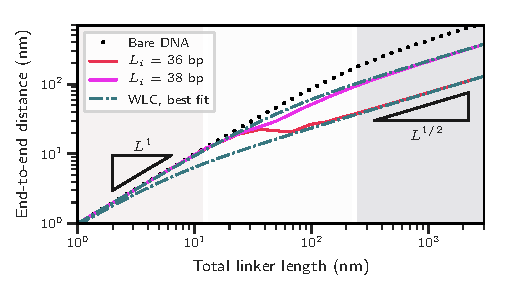
\includegraphics{./figures/fig2a_r2_homogenous_vs_wlc.pdf}
    }\\
    \subfloat[]{\label{fig:homo-kuhn-zoom}
        \includegraphics{./figures/fig2b_kuhns31to51_chains.png}
        %TODO add "<L_i>" to xlabel
    }%
    \caption{\protect\subref{fig:r2-homo-wlc} Average end-to-end distance of a
    homogeneous chromatin chain with 36bp linkers, as compared to the best-fit
    wormlike chains in the short and long length regimes.
    \protect\subref{fig:homo-kuhn-zoom} Kuhn lengths of homogeneous chromatin
    chains are 10.5bp periodic in linker length. Example minimum energy chain
    configurations are shown. Compact structures (36, \SI{47}{\basepair}) afford
    more flexibility than more processive structures (\SI{41}{\basepair}), which
    have higher Kuhn lengths.}\label{fig:homo-chain}
\end{figure}

%TODO make clear that the zero temperature picture is the depicted chains, and
%the plot is the fluctuating case, make super sure this is more clear
To build a geometric intuition for how the kinks create this modified Kuhn
    length, we compare the Kuhn lengths of various chains to their
    zero-temperature configurations, where the entire chain is composed of
    rigid-rod linkers.
Figure~\ref{fig:homo-kuhn-zoom} shows that the chains with more ``processive''
    zero-temperature structures are exactly those with larger Kuhn lengths.
More precisely, every homogeneous chain at zero temperature forms a
    helix of nucleosomes (as a consequence of Chasles' theorem).
The rise per basepair of the helix is determined by the spherical angles
    $\theta$ and $\phi$ connecting adjacent linkers (see Fig.~\ref{fig:nuc-geo}).
The nucleosome structure fixes $\theta$, but $\phi$ depends linearly on the
    linker length, and is \SI{10.5}{\basepair} periodic due to the DNA helicity.
Select values of $\phi$ lead to more compact zero-temperature structures with a
    smaller rise per basepair.
By extension, the corresponding fluctuating structures have smaller Kuhn lengths.

In Fig.~\ref{fig:homo-kuhn-zoom}, we see that the periodicity in $\phi$ determines the \SI{10.5}{\basepair} periodicity of the Kuhn
    length as a function of linker length.
For long linkers ($L_i\to\infty$), the Kuhn length approaches that of
    bare DNA (Supplemental Fig.~S5).
However, this approach is power-law slow, since the kink density decreases as $1/L_i$, and is largely imperceptible for experimentally relevant linker lengths.

\begin{figure}
    \centering
    \includegraphics{./figures/fig3_kuhns_sigma0to40_chains.png}
    %TODO add verbal definition of sigma to xlabel
    %TODO maybe put the actual uniform phi in this plot instead for dotted line
    \caption{Kuhn length of a heterogeneous chromatin chain with uniformly
    distributed linker lengths chosen from the range $\mu \pm \sigma$, where
    $\mu = \SI{41}{\basepair}$. Example zero-temperature chains composed of rigid
    rod linkers are shown for $\sigma = 0, 2, \SI{6}{\basepair}$. Kuhn length
    rapidly approaches that of a chain drawn from the maximum entropy
    distribution, in which linker lengths are exponentially distributed about
    the same $\mu$. In this universal limit, the minimum energy structure is a
    random walk.}\label{fig:hetero-geom}
\end{figure}

%% what determines zero temperature picture for het chains
We next apply our fluctuating theory to study heterogeneous chains such as those
    in~\cite{woodcock1993}, where the linker lengths are drawn uniformly from a
    range $\mu \pm \sigma$.
In Fig.~\ref{fig:hetero-geom}, we see that as we increase $\sigma$, the
    zero-temperature configuration of the chain interpolates between a helix at
    $\sigma = 0$ and a random walk at larger $\sigma$.
As $\sigma$ increases, the distribution of $\phi \in [0, 2\pi]$ connecting
    adjacent linkers quickly becomes approximately uniform.
As a result, the zero-temperature structure itself has a Kuhn length, which we
    define as ``processivity'' for the case of heterogeneous chains.
As in the homogeneous case, processivity of the zero-temperature chain
    qualitatively predicts that of the fluctuating structure, as seen in
    Fig.~\ref{fig:hetero-geom}.


In the cell, the simplest model of nucleosome binding is the maximum-entropy
    distribution, where nucleosomes bind uniformly randomly along the DNA\@.
For a sufficiently large lattice, the distances separating the nucleosomes in
    this model are well-approximated by an exponential distribution, as implied
    by state-of-the-art models of nucleosome positioning~\cite{beshnova2014}.

In addition, as shown in Fig.~\ref{fig:hetero-geom}, with increasing
    heterogeneity, the Kuhn length converges to that of the freely rotating
    chain (uniform $\phi$, constant bond length) whose bond length matches the
    average.
Because this suggests

In what follows, we use exponentially distributed linker lengths to predict
    behavior of realistic chromatin structures.
Many factors, including histone stacking and sequence-dependent chromatin
    remodelers, will affect the exact linker-length distribution \textit{in vivo}.
However, the distribution-independent convergence of our model as $\phi$ becomes
    uniform means our results are likely robust to these effects.

\begin{figure}
    \centering
    \includegraphics{./figures/fig4b_kuhn_exponential.pdf}
        % add verbal description of xlabel
    \caption{Kuhn lengths of universal chromatin chains with exponentially
    distributed linkers, as a function of the average linker length, which
    varies by cell type. Kuhn lengths for \textit{S. cerevisiae}
    ($\meanli=\SI{15}{\basepair}$), mice embryonic stem cells
    ($\meanli=\SI{45}{\basepair}$), and human T cells
    ($\meanli=\SI{56}{\basepair}$) are marked.}\label{fig:exp-chain}
\end{figure}

%TODO fix wording
Note that the ``exponential chain'' corresponds to a modified freely rotating
    chain.
As has been proven in~\cite{kilanowski2017}, this chain averages to an effective
    TWLC with the same Kuhn length (see Supplemental Figure~S7).
This means that coarse-graining chromatin's structure only requires computing
    the Kuhn length of the exponential chain for the desired $\meanli$, which
    varies based on the cell type.

We present these Kuhn lengths as a function of $\meanli$ in
    Fig.~\ref{fig:exp-chain}.
Because increasing $\meanli$ only scales the random walk, the Kuhn length lacks
    the \SI{10.5}{\basepair} periodicity of the homogeneous chain.
%This means that chromatin's large scale behavior is less sensitive to the nucleosome repeat length than previously predicted in the homogeneous case.
A table of these Kuhn lengths is available in Supplemental Table 1, and we
    emphasize that an approximate knowledge of the nucleosome repeat length should
    be sufficient for coarse-graining.

%% trans to looping
Many biological processes are influenced by the local organization of chromatin,
    which can be characterized by the propensity for genomic loci to form
    chromatin loops.
Our analytical theory is well suited to calculate looping probability, which is an
    extremely rare event in most cases.
We numerically invert the Fourier transform in Eq.~\ref{eq:expansion} to evaluate
    $\greens[L]{\vec{R}}$ at $\vec{R} = 0$.
Note that $P_\text{loop}=\greens[L]{\vec{R}=0}$ corresponds to a modified
    $J$-factor with no orientational component.
In Fig.~\ref{fig:looping}, we plot this probability as a function of the loop size.

\begin{figure}
    \centering
    \includegraphics{./figures/fig5_looping_hetero31to52bp_bold3curves.pdf}
    \caption{Each purple line designates an individual chain configuration with
    uniformly random linker lengths between 31 and \SI{51}{\basepair}, with the
    black line representing the average over individual chains. A wormlike chain
    (red dashed line) with the same Kuhn length as this average chain captures the
    looping probability for loops composed of more than 3--4 nucleosomes. Three
    random individual chains are bolded.}\label{fig:looping}
\end{figure}

Strikingly, we observe that the difference between the most- and least-likely to
    loop loci spans six orders of magnitude.
This huge inter-chain variability is driven by the unique geometrical properties
    of individual chromatin chains (Supplemental Fig.~S7).
As a result, on time scales shorter than nucleosome turnover, loop formation can
    be dramatically influenced by local changes to nucleosome positioning.
In addition, the typical model of chromatin as bare DNA systematically
    underestimates the looping propensity. In other words, rearranging
    nucleosome positions has a more profound effect than bending DNA on the
    looping probability of genomic loci.

For time scales much longer than nucleosome turnover, the best-fit wormlike
    chain is able to capture the probability of DNA contacts as a function of
    genomic separation for distances larger than three nucleosomes.
We note that this change in the effective Kuhn length corresponds to increasing
    the propensity for kilobase-scale loops by over three orders of magnitude.
At longer length scales, the average looping probability approaches that of a
    Gaussian chain with the characteristic $L^{-3/2}$ scaling.
However, individual chains retain memory of rigid kinks, as indicated by
    residual peaks in the looping probability of the highlighted chains.


% \section{\label{sec:discussion}Discussion}

Our model excludes various important facets of chromatin's structure, such as
    steric interactions between nucleosomes that are well known~\cite{widom1992}
    to constrain the space of possible linker lengths.
In addition, our model ignores the finite size of the nucleosome, treating it as
    a point-like kink in the DNA backbone.

%TODO fix wording, mention that model "looks like" chromatin
While the exact quantitative values we predict will change as more detail is
    added, our estimates of Kuhn length and looping probabilities provide
    guidance to future coarse-grained models of chromatin.
We provide rigorous justification for the common practice of using an effective
    TWLC to model \textit{in vivo} chromatin.
On the other hand, we show that the common practice~\cite{macphersonInPress,nuebler2018}
    of using a Kuhn length of \SI{100}{\nano\metre} likely leads to at least a
    four-fold overestimation of the polymer's stiffness.

%TODO wording feels "sudden"
Our model can also incorporate fluctuations in the number of basepairs bound to
    each nucleosome due to nucleosome
% I have tons of citations for these two statements in zotero, just have to
% separate them from each other tediously to make two lists
    breathing~\cite{TODO}, forces on the DNA~\cite{TODO}, or active
    remodelling~\cite{dion2007,kulaeva2007,senavirathne2017}.
%In order to avoid an arbitrary choice of unwrapping distributions, we focused on the constant $\theta$ case.
Nucleosome unwrapping would change the angle $\theta \in [0, \pi]$
    between adjacent nucleosomes, just as the linker length changes
    $\phi$, resulting in an even more random structure.

%TODO helical wormlike chain no longer mentioned elsewhere, fix wording here
It is interesting to note that the helical wormlike chain has been employed
    in the past to explain the looping statistics of bare DNA~\cite{shimada1984,
    liu2011a}.
Along with the ``kinked'' wormlike chain model~\cite{wiggins2005,
    popov2005}---where kinks are flexible, and represent melted base
    pairs---these models were developed to explain the propensity for small DNA
    loops to form \textit{in vivo}.
%TODO make punch-ier
Our model highlights that even without models of DNA more detailed than the
    TWLC, the specific or non-specific binding of any protein to DNA can
    dramatically amplify short-range DNA contacts.\@

\begin{acknowledgements}
Financial support for this work is provided by the National Science Foundation
    (NSF), Physics of Living Systems Program (PHY-1707751). Q.M. and B.B.
    acknowledge funding support from the NSF Graduate Fellowship program
    (DGE-1656518). B.B. acknowledges support from NIH Training Grant
    T32GM008294.
\end{acknowledgements}

\bibliography{chromatin}

\end{document}
